\documentclass[unknownkeysallowed]{beamer}
\usepackage[utf8]{inputenc}
\usepackage[french,english]{babel}
\usepackage{csquotes}
\usepackage{../sty/beamer_js}
\usepackage{../sty/shortcuts_js}

\usepackage{dirtree}
\newcommand{\Benchopt}{\texttt{Benchopt}}
\newcommand{\TutorialRepoURL}{https://github.com/tomMoral/malga_tuto}
\newcommand{\TutorialBenchDir}{\texttt{malga\_tuto/poisson\_deblur}}
\newcommand{\BaseSolver}{\texttt{PGD}}
\newcommand{\NewSolver}{\texttt{MirrorDescent}}
\newcommand{\NewBenchmark}{\texttt{blind\_deblur}}

% -----------------------------------------------------------------------------
% RETARGETING NOTES (for another tutorial repo/benchmark)
% 1) Update these macros first:
%    - \TutorialRepoURL
%    - \TutorialBenchDir
%    - \BaseSolver / \NewSolver
%    - \NewBenchmark
% 2) Update install/run commands in the "Install and run the benchmark" frame.
% 3) Update the file paths and metric names in:
%    - "What happens during install and run?"
%    - Solver Step 3 validation checklist
%    - New benchmark Step 2 protocol changes
% 4) Update benchmark-specific solver filenames in "Step 3: add solvers and
%    validate" for the new benchmark section.
% -----------------------------------------------------------------------------

\definecolor{tomcolor}{rgb}{0.,.3,.6}
\lstset{basicstyle=\color{tomcolor}\scriptsize\ttfamily}
\addbibresource{../biblio/biblio.bib}
\begin{document}

%%%%%%%%%%%%%%%%%%%%%%%%%%%%%%%%%%%%%%%%%%%%%%%%%%%%%%%%%%%%%%%%%%%%%%%%%%%%%%%
%%%%%%%%%%%%%%%%%%%%%%             Headers               %%%%%%%%%%%%%%%%%%%%%%
%%%%%%%%%%%%%%%%%%%%%%%%%%%%%%%%%%%%%%%%%%%%%%%%%%%%%%%%%%%%%%%%%%%%%%%%%%%%%%%


%%%%%%%%%%%%%%%%%%%%%%%%%%%%%%%%%%%%%%%%%%%%%%%%%%%%%%%%%%%%%%%%%%%%%%%%%%%%%%%
\begin{frame}
\bigskip
\bigskip
\begin{center}{
\LARGE\color{marron}
\textbf{\texttt{Benchopt}:\\
Reproducible, efficient, and collaborative optimization benchmarks}
\textbf{ }\\
}

\color{marron}
\end{center}

\vspace{0.5cm}

\begin{center}
\textbf{Benchopt contributors} \\
\vspace{0.1cm}
\url{https://benchopt.github.io}\\
\end{center}

\centering

\includegraphics[width=0.43\textwidth]{../sharedimages/benchopt_logo.pdf}

\end{frame}
%%%%%%%%%%%%%%%%%%%%%%%%%%%%%%%%%%%%%%%%%%%%%%%%%%%%%%%%%%%%%%%%%%%%%%%%%%%%%%%

% %%%%%%%%%%%%%%%%%%%%%%%%%%%%%%%%%%%%%%%%%%%%%%%%%%%%%%%%%%%%%%%%%%%%%%%%%%%%%%%
% \begin{frame}{Contributors from...}
%     \centering
%     
\includegraphics[width=100px]{../sharedimages/logo_inria_horiz.pdf} \hspace{1mm}
%     \includegraphics[height=45px]{../sharedimages/um_logo.pdf} \hspace{1mm}
%     
\includegraphics[height=35px]{../sharedimages/logo_berkeley.png} \hspace{1mm}
%     \\[7mm]
%     
\includegraphics[height=50px]{../sharedimages/logo_cnrs.pdf} \hspace{5mm}
%     
\includegraphics[height=50px]{../sharedimages/logo_lund} \hspace{5mm}
%     
\includegraphics[height=50px]{../sharedimages/logo_telecom.pdf} \hspace{5mm}
%     
\includegraphics[height=50px]{../sharedimages/logo_univ_luxembourg.pdf} \\[4mm]
%     
\includegraphics[height=40px]{../sharedimages/logo_ens.png}
%     % \includegraphics[height=40px]{../sharedimages/}
% \end{frame}
% %%%%%%%%%%%%%%%%%%%%%%%%%%%%%%%%%%%%%%%%%%%%%%%%%%%%%%%%%%%%%%%%%%%%%%%%%%%%%%%



%%%%%%%%%%%%%%%%%%%%%%%%%%%%%%%%%%%%%%%%%%%%%%%%%%%%%%%%%%%%%%%%%%%%%%%%%%%%%%%
\begin{frame}{Why benchmarks matter}

    Benchmarks are central to empirical progress in ML:\\[.5em]
    \begin{itemize}
        \item They define what we compare and report.
        \item They make progress measurable across papers.
        \item They provide the baselines used by the whole community.
    \end{itemize}

    \pause
    \vskip2em
    \strongpoint{No reliable benchmark, no reliable scientific claim in ML.}

\end{frame}
%%%%%%%%%%%%%%%%%%%%%%%%%%%%%%%%%%%%%%%%%%%%%%%%%%%%%%%%%%%%%%%%%%%%%%%%%%%%%%%

%%%%%%%%%%%%%%%%%%%%%%%%%%%%%%%%%%%%%%%%%%%%%%%%%%%%%%%%%%%%%%%%%%%%%%%%%%%%%%%
\begin{frame}{The hidden cost of benchmarking}

    Different teams often rebuild the same engineering stack:\\[.5em]
    \begin{itemize}
        \item Install and environment creation.
        \item Dependency management and data preparation.
        \item Run orchestration, evaluation and plotting.
    \end{itemize}

    \vskip1.5em
    \strongpoint{Repeated tooling slows down science and creates avoidable burden.}

\end{frame}
%%%%%%%%%%%%%%%%%%%%%%%%%%%%%%%%%%%%%%%%%%%%%%%%%%%%%%%%%%%%%%%%%%%%%%%%%%%%%%%




%%%%%%%%%%%%%%%%%%%%%%%%%%%%%%%%%%%%%%%%%%%%%%%%%%%%%%%%%%%%%%%%%%%%%%%%%%%%%%%
\begin{frame}{What \Benchopt{} changes}

    \Benchopt{} factorizes the common benchmark tooling:\\[.5em]
    \begin{itemize}
        \item Standard interfaces: objective, dataset, solver.
        \item Reusable workflow: install, run, test, compare, share.
        \item Run anywhere: explicit dependencies and controlled environments.
        \item Reliable reruns: controlled randomness and reproducible protocols.
        \item New in recent releases: merge runs and publish to GitHub/Hugging Face.
    \end{itemize}

    \pause
    \vskip1.5em
    \strongpoint{Benchopt does not replace benchmarks,\\it removes duplicated plumbing.}

\end{frame}
%%%%%%%%%%%%%%%%%%%%%%%%%%%%%%%%%%%%%%%%%%%%%%%%%%%%%%%%%%%%%%%%%%%%%%%%%%%%%%%


%%%%%%%%%%%%%%%%%%%%%%%%%%%%%%%%%%%%%%%%%%%%%%%%%%%%%%%%%%%%%%%%%%%%%%%%%%%%%%%
\begin{frame}{Benchopt scope}

    \Benchopt{} turns benchmark code into reusable research infrastructure.
    \vskip1.5em

    {\centering
    \vskip2em
    {\Large\Benchopt{} produces \textbf{open}, \textbf{reproducible}, \textbf{extendable} benchmarks.}\\
    }
    \vskip1em
    \begin{itemize}
        \item Comparable and fairer evaluations,
        \item Faster iterations on methods and datasets,
        \item Lower engineering overhead across projects.
    \end{itemize}

    \vskip1.2em
    {\centering And keeps them \textbf{maintainable} through explicit interfaces\\and tests.\\}

\end{frame}
%%%%%%%%%%%%%%%%%%%%%%%%%%%%%%%%%%%%%%%%%%%%%%%%%%%%%%%%%%%%%%%%%%%%%%%%%%%%%%%



%%%%%%%%%%%%%%%%%%%%%%%%%%%%%%%%%%%%%%%%%%%%%%%%%%%%%%%%%%%%%%%%%%%%%%%%%%%%%%%
\begin{frame}{Extra tools for easier benchmarking}

    \begin{itemize}
        \item \textbf{Integrate broadly:} use implementations from Python, R, Julia, or binaries.
        \item \textbf{Scale experiments:} run in parallel locally or on distributed backends.
        \item \textbf{Save time:} cache results to avoid recomputing unchanged runs.
        \item \textbf{Trust comparisons:} control randomness with seeds and stable protocols.
        \item \textbf{Share outcomes:} merge and publish results from multiple runs, easy visualization.
    \end{itemize}

    \vskip0.7em
    \centering
    
\includegraphics[width=0.8\linewidth]{../sharedimages/tweet_rahimi.png}

\end{frame}
%%%%%%%%%%%%%%%%%%%%%%%%%%%%%%%%%%%%%%%%%%%%%%%%%%%%%%%%%%%%%%%%%%%%%%%%%%%%%%%



%%%%%%%%%%%%%%%%%%%%%%%%%%%%%%%%%%%%%%%%%%%%%%%%%%%%%%%%%%%%%%%%%%%%%%%%%%%%%%%
\begin{frame}{How does \Benchopt{} do it?}

\Benchopt{} provides a framework to organize and run benchmarks:
\begin{itemize}
    \item Each benchmark is a repository
    \item \Benchopt{} is a \texttt{Python} CLI to install, run, test and share them
\end{itemize}

\vskip1em
Examples of existing benchmarks:
\vskip.5em
\begin{minipage}{0.5\linewidth}
    {\small
    \begin{itemize}
        \item \href{https://github.com/benchopt/benchmark_resnet_classif}{\bf Image Classification (resnet)}
        \item \href{https://github.com/benchopt/benchmark_logreg_l2}{\bf Logistic regression}
        \item \href{https://github.com/benchopt/benchmark_lasso}{\bf Lasso}
        \item \href{https://github.com/benchopt/benchmark_linear_ica}{\bf ICA}
    \end{itemize}
    }
\end{minipage}
\begin{minipage}{0.48\linewidth}
    {\small
    \begin{itemize}
        \item \href{https://github.com/benchopt/benchmark_tv_1d}{\bf Total Variation}
        \item \href{https://github.com/benchopt/benchmark_bilevel}{\bf Bilevel Optimization}
        \item \href{https://github.com/benchopt/benchmark_bci}{\bf Brain Computer Interface}
        \item \href{https://github.com/benchopt/?q=benchmark_&type=all&language=&sort=name}{\bf \dots}
    \end{itemize}
    }
\end{minipage}
\vskip2em

\centering
Start yours with \url{https://github.com/benchopt/template_benchmark} or \url{https://github.com/benchopt/template_benchmark_ml}!
\end{frame}
%%%%%%%%%%%%%%%%%%%%%%%%%%%%%%%%%%%%%%%%%%%%%%%%%%%%%%%%%%%%%%%%%%%%%%%%%%%%%%%


% -----------------------------------------------------------------------------
% TIMING NOTES (15 min)
% - 2 min: Why Benchopt (problem + value proposition)
% - 4 min: Run an existing benchmark (install + first run)
% - 4 min: Add a new solver (PGD -> MirrorDescent)
% - 4 min: Create a new benchmark (blind_deblur)
% - 1 min: Resources + call-to-action + questions
%
% IF SHORT ON TIME
% - Keep: install/run workflow + 3 solver steps + 3 new-benchmark steps
% - Skip: Components/Flow/Structure details + long benchmark example list
% -----------------------------------------------------------------------------



%%%%%%%%%%%%%%%%%%%%%%%%%%%%%%%%%%%%%%%%%%%%%%%%%%%%%%%%%%%%%%%%%%%%%%%%%%%%%%%
\begin{frame}{Tutorial}

    \centering
    \huge Running a benchmark!

\end{frame}
%%%%%%%%%%%%%%%%%%%%%%%%%%%%%%%%%%%%%%%%%%%%%%%%%%%%%%%%%%%%%%%%%%%%%%%%%%%%%%%


%%%%%%%%%%%%%%%%%%%%%%%%%%%%%%%%%%%%%%%%%%%%%%%%%%%%%%%%%%%%%%%%%%%%%%%%%%%%%%%
\begin{frame}[fragile]{Install and run the benchmark}

    \textbf{Repository used in the tutorial:}\\[.3em]
    \url{\TutorialRepoURL}

    \vskip1em
    \textbf{Minimal workflow:}

\begin{lstlisting}[language=bash]
git clone https://github.com/tomMoral/malga_tuto.git
cd malga_tuto/poisson_deblur
pip install benchopt
benchopt install .
benchopt run .
\end{lstlisting}

    \vskip0.7em
    \strongpoint{Once \Benchopt{} is installed, two commands are enough: install the benchmark, then run it.}

\end{frame}
%%%%%%%%%%%%%%%%%%%%%%%%%%%%%%%%%%%%%%%%%%%%%%%%%%%%%%%%%%%%%%%%%%%%%%%%%%%%%%%


%%%%%%%%%%%%%%%%%%%%%%%%%%%%%%%%%%%%%%%%%%%%%%%%%%%%%%%%%%%%%%%%%%%%%%%%%%%%%%%
\begin{frame}{What happens during install and run?}

    For this benchmark, \Benchopt{} will automatically:\\[.5em]
    \begin{itemize}
        \item Load the objective, dataset and available solvers.
        \item Install the benchmark requirements declared in the files.
        \item Run the available solver on the \texttt{TubLevel} dataset.
        \item Collect metrics such as \texttt{psnr} and \texttt{ssim}.
    \end{itemize}

    \vskip1.2em
    \textbf{In this repo:}
    \begin{itemize}
        \item Dataset file: \texttt{datasets/tub\_level.py}
        \item Objective: \texttt{objective.py}
        \item First solver: \texttt{solvers/pgd.py}
    \end{itemize}

\end{frame}
%%%%%%%%%%%%%%%%%%%%%%%%%%%%%%%%%%%%%%%%%%%%%%%%%%%%%%%%%%%%%%%%%%%%%%%%%%%%%%%


%%%%%%%%%%%%%%%%%%%%%%%%%%%%%%%%%%%%%%%%%%%%%%%%%%%%%%%%%%%%%%%%%%%%%%%%%%%%%%%
\begin{frame}{Components of a benchmark}

    \centering
    \vspace*{-5mm}
    \textbf{3 components}: Objective, Dataset, Solver

    \vskip3em
    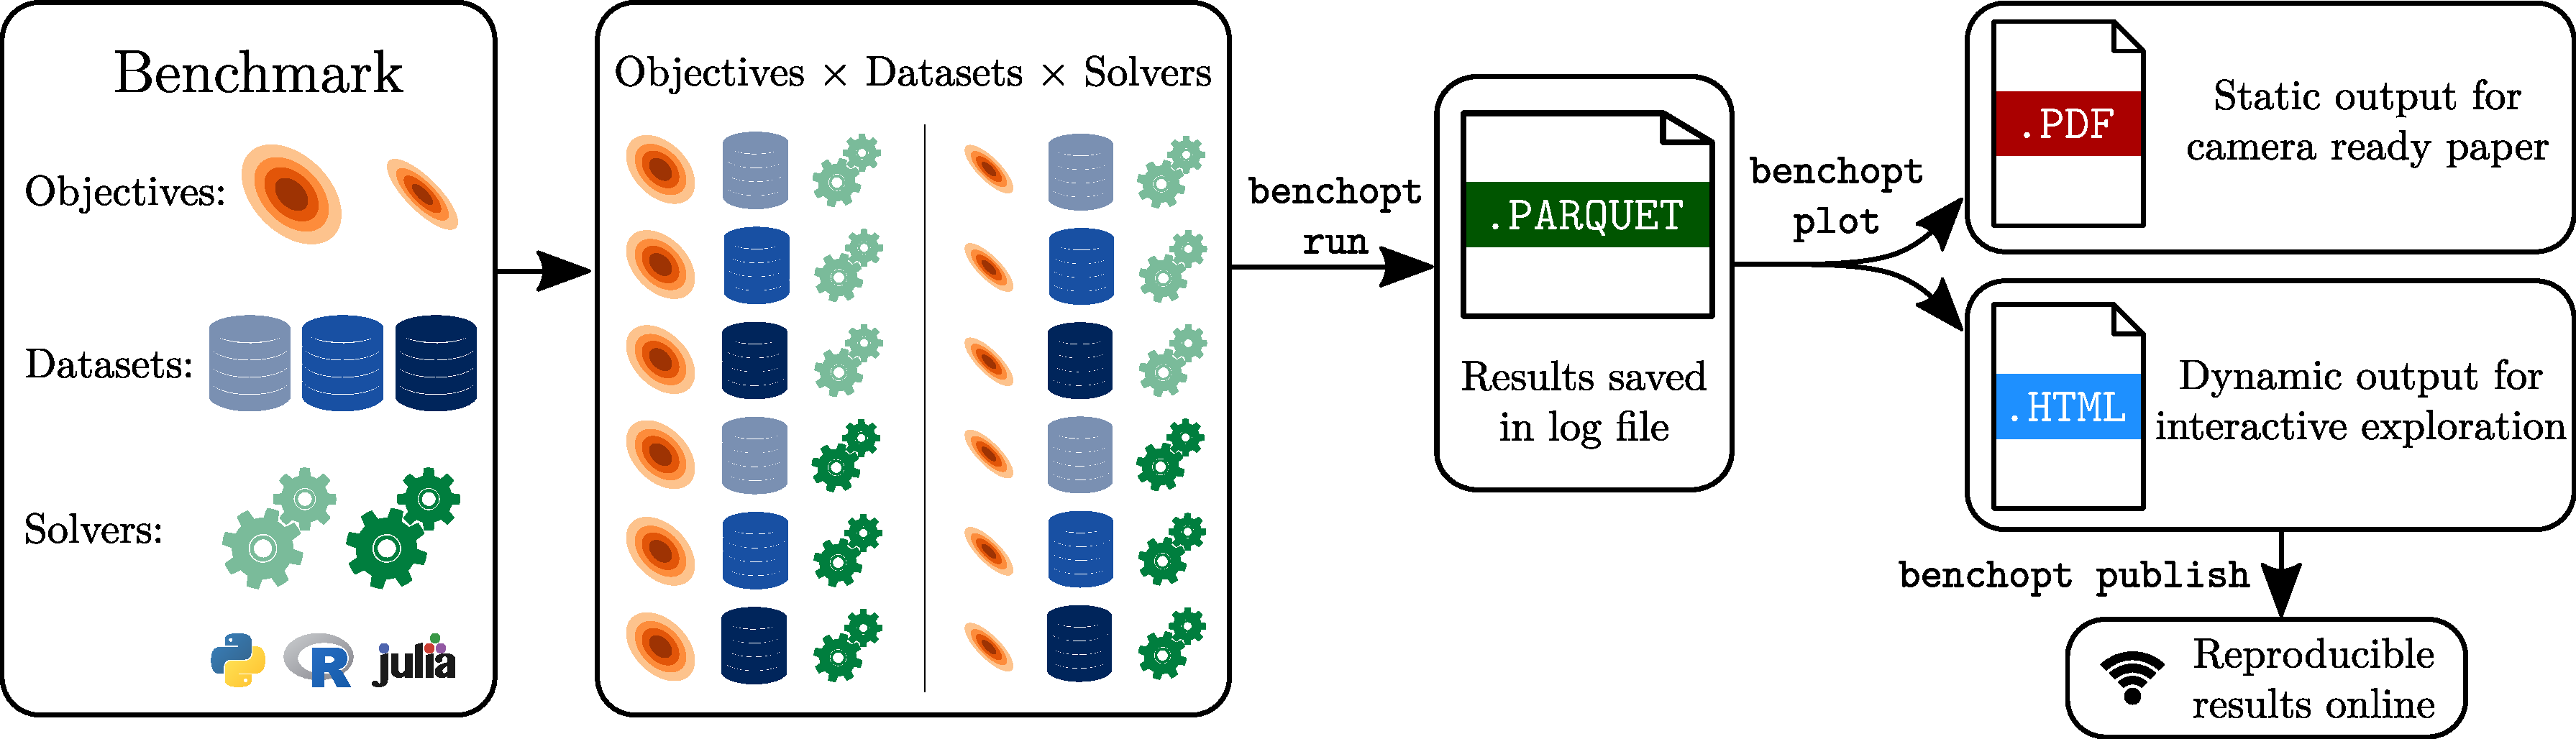
\includegraphics[width=\linewidth]{../sharedimages/benchopt_schema.pdf}

\end{frame}
%%%%%%%%%%%%%%%%%%%%%%%%%%%%%%%%%%%%%%%%%%%%%%%%%%%%%%%%%%%%%%%%%%%%%%%%%%%%%%%


%%%%%%%%%%%%%%%%%%%%%%%%%%%%%%%%%%%%%%%%%%%%%%%%%%%%%%%%%%%%%%%%%%%%%%%%%%%%%%%
\begin{frame}{Flow of a benchmark}

    \centering
    \vspace*{-5mm}
    \textbf{3 components}: Objective, Dataset, Solver

    \vskip3em
    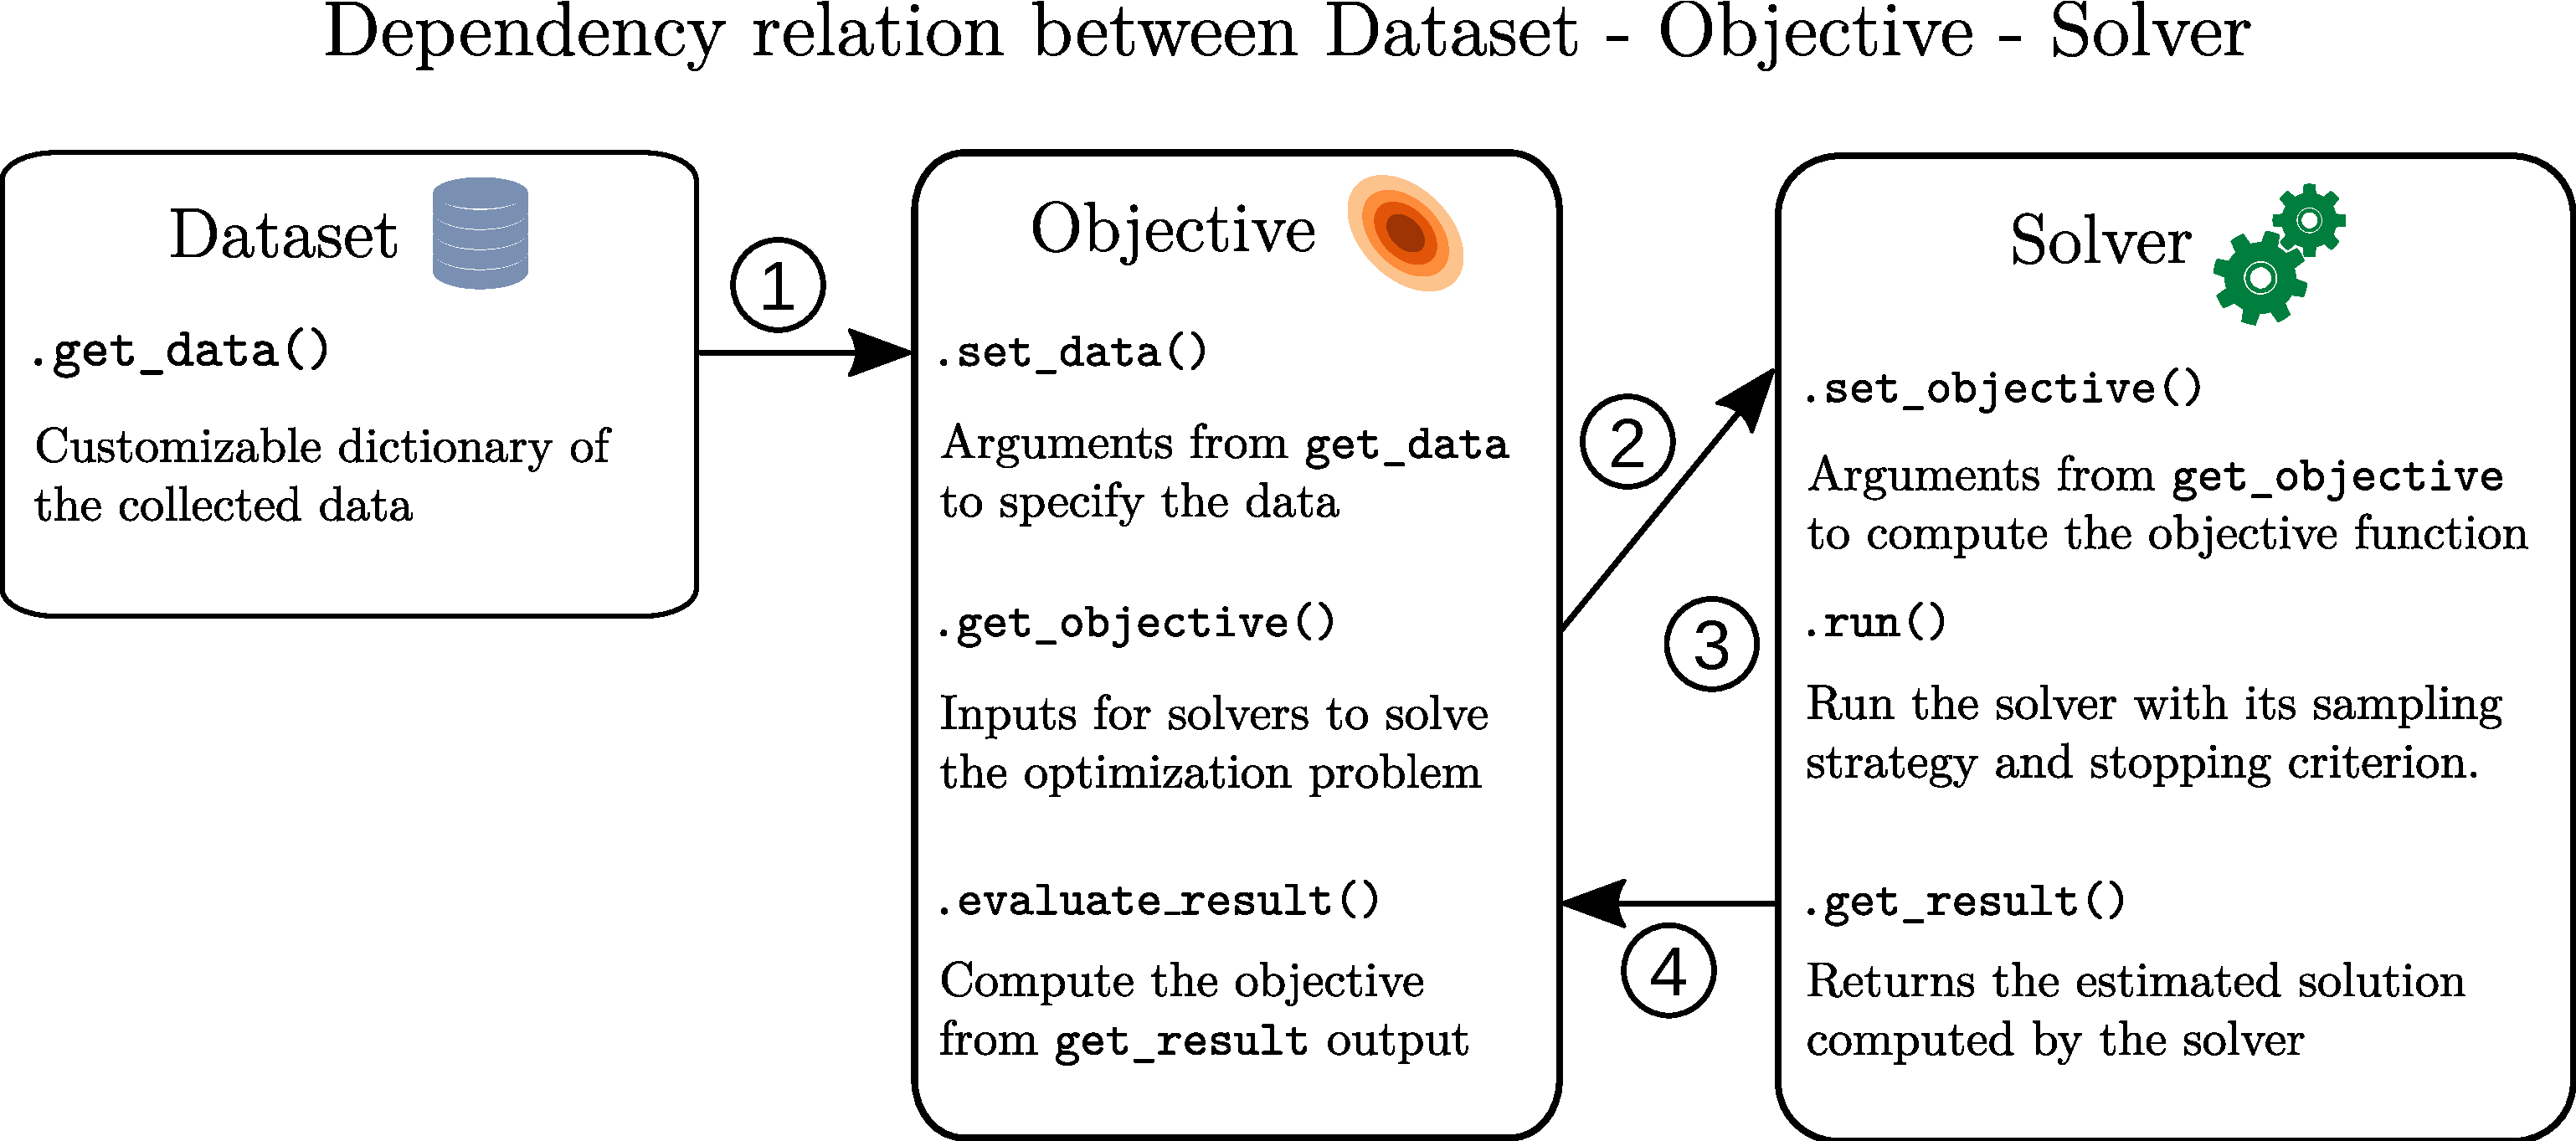
\includegraphics[width=\linewidth]{../sharedimages/benchopt_schema_dependency.pdf}

\end{frame}
%%%%%%%%%%%%%%%%%%%%%%%%%%%%%%%%%%%%%%%%%%%%%%%%%%%%%%%%%%%%%%%%%%%%%%%%%%%%%%%


%%%%%%%%%%%%%%%%%%%%%%%%%%%%%%%%%%%%%%%%%%%%%%%%%%%%%%%%%%%%%%%%%%%%%%%%%%%%%%%
\begin{frame}{Structure of a benchmark}

    \begin{minipage}{0.45\linewidth}
        \dirtree{%
        .1 benchmark/.
        .2 objective.py.
        .2 datasets/.
        .3 dataset1.py.
        .3 dataset2.py.
        .2 solvers/.
        .3 solver1.py.
        .3 solver2.py.
    }
    \end{minipage}
    \begin{minipage}{0.45\linewidth}

    \textbf{Modular \& extendable}
    \vspace*{5mm}

    New solver? add a file

    New dataset? add a file

    New metric? modify objective
    \end{minipage}

\end{frame}
%%%%%%%%%%%%%%%%%%%%%%%%%%%%%%%%%%%%%%%%%%%%%%%%%%%%%%%%%%%%%%%%%%%%%%%%%%%%%%%


%%%%%%%%%%%%%%%%%%%%%%%%%%%%%%%%%%%%%%%%%%%%%%%%%%%%%%%%%%%%%%%%%%%%%%%%%%%%%%%
\begin{frame}{Tutorial}

    \centering
    \huge Adding a solver to an existing benchmark!

\end{frame}
%%%%%%%%%%%%%%%%%%%%%%%%%%%%%%%%%%%%%%%%%%%%%%%%%%%%%%%%%%%%%%%%%%%%%%%%%%%%%%%


%%%%%%%%%%%%%%%%%%%%%%%%%%%%%%%%%%%%%%%%%%%%%%%%%%%%%%%%%%%%%%%%%%%%%%%%%%%%%%%
\begin{frame}[fragile]{Step 1: add a new solver file}

    \textbf{Goal:} add one more method without changing the benchmark protocol.

    \vskip1em
    \begin{itemize}
        \item Create a new file: \texttt{solvers/mirror\_descent.py}
        \item Start from \texttt{solvers/pgd.py} rather than from scratch
        \item Rename the solver to \NewSolver{}
        \item Keep the same parameters and \texttt{sampling\_strategy}
        \item Reuse the same objective inputs and helper losses
    \end{itemize}

    \strongpoint{Same interface, same objective, same dataset: only the method changes.}

\end{frame}
%%%%%%%%%%%%%%%%%%%%%%%%%%%%%%%%%%%%%%%%%%%%%%%%%%%%%%%%%%%%%%%%%%%%%%%%%%%%%%%


%%%%%%%%%%%%%%%%%%%%%%%%%%%%%%%%%%%%%%%%%%%%%%%%%%%%%%%%%%%%%%%%%%%%%%%%%%%%%%%
\begin{frame}[fragile]{Step 2: change the optimization logic}

    Reuse the same objective inputs in \texttt{set\_objective}:\\[.3em]
    \texttt{y}, \texttt{physics}, \texttt{back}, and the same helper losses.

    \vskip1em
    \textbf{PGD update}
    $$
    x_{k+1} = \max\left(x_k - \tau \nabla f(x_k), 0\right)
    $$

    \textbf{Mirror descent update}
    $$
    x_{k+1} = \frac{x_k}{1 + \tau x_k \nabla f(x_k)}
    $$

    \strongpoint{Also need to update $\tau$ computation.}

\end{frame}
%%%%%%%%%%%%%%%%%%%%%%%%%%%%%%%%%%%%%%%%%%%%%%%%%%%%%%%%%%%%%%%%%%%%%%%%%%%%%%%


%%%%%%%%%%%%%%%%%%%%%%%%%%%%%%%%%%%%%%%%%%%%%%%%%%%%%%%%%%%%%%%%%%%%%%%%%%%%%%%
\begin{frame}[fragile]{Step 3: validate the new solver}

    Benchopt will automatically compare the new solver to the existing one.

    \vskip1em
\begin{lstlisting}[language=bash]
benchopt test . -k mirrordescent --skip-env
benchopt run .
\end{lstlisting}

    \vskip0.7em
    What to check:
    \begin{itemize}
        \item The solver is discovered automatically from the new file.
        \item It returns \texttt{x\_hat} in \texttt{get\_result}.
        \item The objective evaluates it with \texttt{psnr} and \texttt{ssim}.
        \item The comparison runs without touching datasets or the objective.
    \end{itemize}

    \vskip0.7em
    \strongpoint{Adding a solver in \Benchopt{} means implementing one compatible file, not rewiring the benchmark.}

\end{frame}
%%%%%%%%%%%%%%%%%%%%%%%%%%%%%%%%%%%%%%%%%%%%%%%%%%%%%%%%%%%%%%%%%%%%%%%%%%%%%%%



%%%%%%%%%%%%%%%%%%%%%%%%%%%%%%%%%%%%%%%%%%%%%%%%%%%%%%%%%%%%%%%%%%%%%%%%%%%%%%%
\begin{frame}{Tutorial}

    \centering
    \huge Creating a new benchmark!

\end{frame}
%%%%%%%%%%%%%%%%%%%%%%%%%%%%%%%%%%%%%%%%%%%%%%%%%%%%%%%%%%%%%%%%%%%%%%%%%%%%%%%


%%%%%%%%%%%%%%%%%%%%%%%%%%%%%%%%%%%%%%%%%%%%%%%%%%%%%%%%%%%%%%%%%%%%%%%%%%%%%%%
\begin{frame}{Step 1: start from an existing benchmark}

    \textbf{Goal:} reuse the previous benchmark and only change what is specific
    to blind deblurring.

    \vskip1em
    \begin{itemize}
        \item Copy the \texttt{poisson\_deblur} benchmark into a new folder
        \item Rename the benchmark and update the \texttt{README.rst}
        \item Keep the same global Benchopt structure:
              \texttt{objective.py}, \texttt{datasets/}, \texttt{solvers/}
        \item Keep the same workflow: \texttt{benchopt test}, then \texttt{benchopt run}
    \end{itemize}

    \vskip1em
    \strongpoint{Creating a new benchmark often starts by\\modifying a nearby one or an existing template,\\not by starting from an empty repo.}

\end{frame}
%%%%%%%%%%%%%%%%%%%%%%%%%%%%%%%%%%%%%%%%%%%%%%%%%%%%%%%%%%%%%%%%%%%%%%%%%%%%%%%


%%%%%%%%%%%%%%%%%%%%%%%%%%%%%%%%%%%%%%%%%%%%%%%%%%%%%%%%%%%%%%%%%%%%%%%%%%%%%%%
\begin{frame}{Step 2: adapt the benchmark protocol}

    Compared to \texttt{poisson\_deblur}, the main changes are:

    \vskip1em
    \begin{itemize}
        \item New task: recover both the image $x$ and the blur kernel $k$
        \item New dataset: generate blurry observations from \texttt{Set3C}
        \item New objective signature: evaluate \texttt{x\_hat} and \texttt{k\_hat}
        \item New metric: add \texttt{kernel\_mse} in addition to \texttt{psnr}
    \end{itemize}

    \vskip1em
    Concretely, most of the work is in:
    \begin{itemize}
        \item \texttt{datasets/set3c\_blur.py}
        \item \texttt{objective.py}
    \end{itemize}

\end{frame}
%%%%%%%%%%%%%%%%%%%%%%%%%%%%%%%%%%%%%%%%%%%%%%%%%%%%%%%%%%%%%%%%%%%%%%%%%%%%%%%


%%%%%%%%%%%%%%%%%%%%%%%%%%%%%%%%%%%%%%%%%%%%%%%%%%%%%%%%%%%%%%%%%%%%%%%%%%%%%%%
\begin{frame}[fragile]{Step 3: add solvers and validate}

    Once the protocol is defined, add benchmark-specific solvers.

    \vskip1em
    In this example:
    \begin{itemize}
        \item \texttt{solvers/bilevel.py} for a bilevel baseline
        \item \texttt{solvers/dip\_selfdeblur.py} for a DIP/SelfDeblur approach
        \item \texttt{benchmark\_utils/networks.py} for shared neural network blocks
    \end{itemize}

    \vskip1em
\begin{lstlisting}[language=bash]
benchopt test . --skip-env
benchopt run .
\end{lstlisting}

    \vskip0.7em
    \strongpoint{A new benchmark means defining a new protocol, then plugging methods into the same Benchopt workflow.}

\end{frame}
%%%%%%%%%%%%%%%%%%%%%%%%%%%%%%%%%%%%%%%%%%%%%%%%%%%%%%%%%%%%%%%%%%%%%%%%%%%%%%%


%%%%%%%%%%%%%%%%%%%%%%%%%%%%%%%%%%%%%%%%%%%%%%%%%%%%%%%%%%%%%%%%%%%%%%%%%%%%%%%
\begin{frame}{\Benchopt{} Roadmap}
    \begin{itemize}\itemsep1em
        \item \textbf{Simpler solver evaluation --} make custom solver integration more direct, for instance with \texttt{eval\_solver(run\_func)}
        \item \textbf{Better visualization tools -- } explore results more easily, in particular for image tasks
        \item \textbf{More reference benchmarks --} grow the benchmark collection with community contributions
    \end{itemize}


    \strongpoint{\Benchopt{} is by no means finished or complete!}

    \vskip2em
    It is useful to a growing group of people but we need to gather more feedbacks to fit the needs of the community.\\[2em]
\end{frame}
%%%%%%%%%%%%%%%%%%%%%%%%%%%%%%%%%%%%%%%%%%%%%%%%%%%%%%%%%%%%%%%%%%%%%%%%%%%%%%%


%%%%%%%%%%%%%%%%%%%%%%%%%%%%%%%%%%%%%%%%%%%%%%%%%%%%%%%%%%%%%%%%%%%%%%%%%%%%%%%
\begin{frame}{Benchopt links and resources}

    \begin{columns}[T]
        \column{.5\textwidth}
        \vskip1em
        \begin{itemize}\itemsep1em
            \item Documentation:\\ \href{https://benchopt.github.io}{benchopt.github.io}
            \item Main repository: \href{https://github.com/benchopt/benchopt}{github.com/benchopt/benchopt}
            \item Benchmark templates: \href{https://github.com/benchopt/template_benchmark}{github.com/benchopt/template\_benchmark}\\
            \href{https://github.com/benchopt/template_benchmark_ml}{github.com/benchopt/template\_benchmark\_ml}
        \end{itemize}

        \column{.36\textwidth}
        \centering
        \includegraphics[width=.8\textwidth]{qr_benchopt_repos.png}\\[.5em]
    \end{columns}
    \vskip1.2em
    \strongpoint{If this tutorial was useful, please star the \texttt{benchopt} repo and share it.}

\end{frame}
%%%%%%%%%%%%%%%%%%%%%%%%%%%%%%%%%%%%%%%%%%%%%%%%%%%%%%%%%%%%%%%%%%%%%%%%%%%%%%%

\end{document}
